% ============================================================================
% DÉFINITION DU COURS 06 : CORRECTION DES SYSTÈMES ASSERVIS
% ============================================================================

\titlehead{Thomas Lusseau - SII en ATS}
\title[Correction des systèmes asservis]{Correction et réglage des systèmes asservis}
\author[TL]{Thomas Lusseau}
\date{\today}

\TLCourseCoverSetup
  {\repStyle/FondPoly.png}
  {pandoc/images/image3.jpeg}
  {Cycle 3 : Concevoir et régler la commande\\ d'un système asservi}
  {Correction et réglage\\ des systèmes asservis}
  {Lycée Robert Doisneau - ATS}
  {Thomas Lusseau}

\TLCourseCoverContents{%
  \TLCourseContentsLine{6.1}{Introduction à la correction}{introduction-uxe0-la-correction}
  \TLCourseContentsLine{6.2}{Actions proportionnelle, intégrale et dérivée}{diffuxe9rentes-actions-de-correction}
  \TLCourseContentsLine{6.3}{Correcteur proportionnel P}{correcteur-proportionnel-p}
  \TLCourseContentsLine{6.4}{Correcteurs I et PI}{correcteur-intuxe9gral-i}
  \TLCourseContentsLine{6.5}{Retard de phase}{retard-de-phase-ou-correcteur-pi-ruxe9el}
  \TLCourseContentsLine{6.6}{Avance de phase}{correcteur-uxe0-avance-de-phase-ou-correcteur-pd-ruxe9el}
  \TLCourseContentsLine{6.7}{Correcteur PID}{correcteur-proportionnel-intuxe9gral-duxe9rivuxe9-pid}
  \TLCourseContentsLine{6.8}{Bilan et boucles imbriquées}{bilan-des-performances-des-correcteurs}
  \TLCourseContentsLine{6.9}{Exercices du chapitre}{exercices-correction-sa}
}

\TLCourseFooter
\TLCourseCover
\markboth{Correction des systèmes asservis}{Correction des systèmes asservis}
\TLSetReflectionImage{pandoc/images/image5.png}

\AtBeginEnvironment{corrige}{\small}
\livrettrue
\collefalse

\setcounter{chapter}{5}
\chapter*{Correction et réglage des systèmes asservis}
\addcontentsline{toc}{chapter}{Correction et réglage des systèmes asservis}

% Couche d'intégration de la conversion Word/Pandoc du cours 06.
% Les sources normalisées restent lisibles ; les images sont sécurisées ici.

\makeatletter
\let\TLSixOriginalIncludeGraphics\includegraphics
\newif\ifTLSixVectorGraphic

\newcommand{\TLSixMissingGraphic}[1]{%
  \begin{tikzpicture}[baseline=(current bounding box.center)]
    \node[
      draw=TLCoverBlue!55,
      rounded corners=1mm,
      fill=TLCoverBlue!4,
      text=TLCoverBlue!80!black,
      align=center,
      font=\sffamily\scriptsize,
      inner sep=2mm,
      text width=27mm
    ] {Illustration vectorielle\\non convertie\\\ttfamily #1};
  \end{tikzpicture}%
}

\newcommand{\TLSixPlaceOriginal}[3]{%
  \ifinner
    \ifdim\linewidth<12mm
      \TLSixOriginalIncludeGraphics[width=8mm,height=8mm,keepaspectratio]{#3}%
    \else
      \adjustbox{max width=.92\linewidth,max totalheight=.68\textheight}{%
        \IfBooleanTF{#1}
          {\TLSixOriginalIncludeGraphics*[#2]{#3}}
          {\TLSixOriginalIncludeGraphics[#2]{#3}}%
      }%
    \fi
  \else
    \par\noindent
    \makebox[\linewidth][c]{%
      \adjustbox{max width=.95\linewidth,max totalheight=.76\textheight}{%
        \IfBooleanTF{#1}
          {\TLSixOriginalIncludeGraphics*[#2]{#3}}
          {\TLSixOriginalIncludeGraphics[#2]{#3}}%
      }%
    }%
    \par\noindent
  \fi
}

\newcommand{\TLSixPlaceConverted}[1]{%
  \ifinner
    \ifdim\linewidth<12mm
      \TLSixOriginalIncludeGraphics[width=8mm,height=8mm,keepaspectratio]{#1}%
    \else
      \adjustbox{max width=.92\linewidth,max totalheight=.68\textheight}{%
        \TLSixOriginalIncludeGraphics[width=\linewidth,height=.68\textheight,keepaspectratio]{#1}%
      }%
    \fi
  \else
    \par\noindent
    \makebox[\linewidth][c]{%
      \adjustbox{max width=.95\linewidth,max totalheight=.76\textheight}{%
        \TLSixOriginalIncludeGraphics[width=\linewidth,height=.74\textheight,keepaspectratio]{#1}%
      }%
    }%
    \par\noindent
  \fi
}

\RenewDocumentCommand{\includegraphics}{s O{} m}{%
  \begingroup
  \filename@parse{#3}%
  \edef\TLSixGraphicExtension{\filename@ext}%
  \edef\TLSixGraphicStem{\filename@area\filename@base}%

  \TLSixVectorGraphicfalse
  \ifdefstring{\TLSixGraphicExtension}{emf}{\TLSixVectorGraphictrue}{}
  \ifdefstring{\TLSixGraphicExtension}{EMF}{\TLSixVectorGraphictrue}{}
  \ifdefstring{\TLSixGraphicExtension}{wmf}{\TLSixVectorGraphictrue}{}
  \ifdefstring{\TLSixGraphicExtension}{WMF}{\TLSixVectorGraphictrue}{}

  \ifTLSixVectorGraphic
    \IfFileExists{\TLSixGraphicStem.pdf}{%
      \TLSixPlaceConverted{\TLSixGraphicStem.pdf}%
    }{%
      \IfFileExists{\TLSixGraphicStem.png}{%
        \TLSixPlaceConverted{\TLSixGraphicStem.png}%
      }{%
        \ifinner
          \TLSixMissingGraphic{\filename@base}%
        \else
          \par\noindent\makebox[\linewidth][c]{\TLSixMissingGraphic{\filename@base}}\par\noindent
        \fi
      }%
    }%
  \else
    \TLSixPlaceOriginal{#1}{#2}{#3}%
  \fi
  \endgroup
}
\makeatother


% Partie cours issue de 10-CorrectionSA2022.docx.
\hypertarget{introduction-uxe0-la-correction}{%
\section{Introduction à la correction}\label{introduction-uxe0-la-correction}}

\hypertarget{exemple}{%
\subsection{Exemple}\label{exemple}}


\includegraphics[width=1.90625in,height=1.27431in]{pandoc/images/image5.png}Prenons l'exemple d'un véhicule automobile et de son conducteur. On constate que~:

\begin{itemize}
\item
  Le conducteur conduit le véhicule en imposant une position du volant, un rapport de vitesses, une position des pédales d'accélérateur et de freins ;
\item
  Le conducteur doit obéir à des critères. Il doit se déplacer d'un point à un autre en minimisant le temps de parcours tout en restant sur la route et tout en respectant les limites de vitesse~;
\item
  Le conducteur acquiert visuellement et tactilement des informations sur la vitesse, la trajectoire du véhicule, la position du volant\ldots~;
\item
  Le conducteur évalue ces différents paramètres pour élaborer et modifier la conduite du véhicule.
\end{itemize}

L'ensemble correspond à un système asservi où le conducteur, tel un capteur, complète la boucle de retour, joue le rôle de comparateur et celui du bloc élaborant la commande.

Si le temps de parcours est jugé trop long, on peut changer le véhicule (le système commandé) pour un autre plus puissant, ou changer le conducteur (le générateur de commande) pour un pilote de rallye. Mais même le meilleur pilote ne pourra pas faire de miracles avec une voiture poussive.

Dans un système asservi, la commande est élaborée de façon autonome à partir de l'écart entre la consigne et la réponse. Pour améliorer les performances, on ajoute un correcteur. Il peut être placé de plusieurs façons~:

\begin{itemize}
\item
  Dans la chaîne directe en série
\item
  Dans une boucle en parallèle avec point de prélèvement en aval~;
\item
  Dans une boucle par anticipation avec point de prélèvement en amont.
\end{itemize}

Nous allons étudier par la suite un correcteur série. Il corrige le système en amont de l'actionneur.

Les 3 actions de base, proportionnelle, intégrale, dérivée, correspondent à 3 modifications réalisables sur une fonction de transfert~:

\begin{itemize}
\item
  Modifier le gain~;
\item
  Ajouter un pôle~;
\item
  Ajouter un zéro.
\end{itemize}

\hypertarget{introduction-aux-correcteurs}{%
\subsection{Introduction aux correcteurs}\label{introduction-aux-correcteurs}}

\TLCorrecteurSerie


Les correcteurs peuvent être placés à différents endroits de notre système (correction série ou cascade, correction parallèle, correction par anticipation, \ldots). Nous n'étudierons ici que les correcteurs de type série ou cascade qui correspondent au schéma suivant. Il peut ainsi corriger les perturbations qui peuvent apparaître dans la chaîne d'énergie.

On peut également utiliser des filtres au niveau de l'entrée ou de la mesure pour améliorer le signal traité par le correcteur.

Le but de la correction est \textbf{d'améliorer les performances} \textbf{d'un système afin de répondre à un cahier des charges donné}. Les critères principaux apparaissant dans un diagramme d'exigence peuvent être alors~:

\begin{longtable}[]{@{}
  >{\raggedright\arraybackslash}p{(\columnwidth - 2\tabcolsep) * \real{0.2085}}
  >{\raggedright\arraybackslash}p{(\columnwidth - 2\tabcolsep) * \real{0.7915}}@{}}
\toprule\noalign{}
\begin{minipage}[b]{\linewidth}\raggedright
\textbf{Critères}
\end{minipage} & \begin{minipage}[b]{\linewidth}\raggedright
\textbf{Caractérisation}
\end{minipage} \\
\midrule\noalign{}
\endhead
\bottomrule\noalign{}
\endlastfoot
Stabilité & Réalisé à partir des marges de gain et de phase \\
Rapidité & Soit à partir du temps de réponse, soit à partir de la bande passante à 0dB de la FTBO puisque les deux sont liés par le temps de réponse réduit \\
Précision & Classe de la FTBO \\
(Dépasssement) & Eventuellement un critère de dépassement limite ou de non dépassement. Ce critère est lié à la stabilité \\
Robustesse & Aptitude du système à vérifier les performances vis-à-vis de perturbations extérieures et/ou d'incertitudes sur le modèle. On parle alors de commande robuste. \\
\end{longtable}

Il faudra toujours garder à l'esprit que le critère principal est bien sûr la stabilité.

On cherchera donc à améliorer~:

\begin{itemize}
\item
  \textbf{La stabilité~:} il faut que notre système soit stable en boucle fermée. On cherchera à avoir un système «~robuste~» avec des marges de gains et de phases élevées.
\item
  \textbf{La précision~:} on veut annuler les écarts jusqu'à un certain ordre (annulation de l'écart d'ordre 1 pour la régulation, écart d'ordre 2 pour la poursuite,\ldots)
\item
  \textbf{La rapidité~}: on veut que le système réagisse le plus rapidement possible (t\textsubscript{r5\%} le plus faible possible)
\item
  \textbf{Limiter le dépassement~:} on veut que le système n'ait pas un dépassement supérieur à n\%
\item
  \textbf{La robustesse :} on veut qu'une incertitude sur le modèle ou une perturnation non prévue, influe peu sur les performances du système.
\end{itemize}

Malheureusement, \textbf{tous ces critères ne peuvent pas être menés de front~}\ldots{} La priorité sera \textbf{toujours d'avoir un système stable}. Il y aura alors des compromis à réaliser (stabilité/rapidité, précision/stabilité,\ldots).

\hypertarget{diffuxe9rentes-actions-de-correction}{%
\subsection{Différentes actions de correction}\label{diffuxe9rentes-actions-de-correction}}

\TLTroisActionsCorrection


Pour corriger notre système, il existe trois actions distinctes qui peuvent être associées. On distingue~:

\begin{itemize}
\item
  \textbf{L'action proportionnelle~«~P~»:} , qui amplifie l'écart \(\epsilon(p)\), améliore la rapidité et la précision mais diminue la stabilité~;
\end{itemize}

\begin{quote}
\[u(t) = K\varepsilon(t) \Rightarrow \boxed{C(p) = K}\]
\end{quote}

Plus K est grand, plus la correction est rapide et la précision élevée mais il peut apparaître un risque d'oscillations.

\begin{itemize}
\item
  \textbf{L'action intégrale~«~I~»:} , qui intègre l'écart \(\epsilon(p)\), améliore la précision mais diminue la rapidité et la stabilité~;
\end{itemize}

\[u(t) = \frac{1}{T_{i}}\int_{0}^{t}{\varepsilon(\tau)d\tau} \Rightarrow \boxed{C(p) = \frac{1}{T_{i}p}}\]

\begin{quote}
Cet effet permet de faire durer l'effet du correcteur tant qu'il subsiste un écart, ce qui favorise le critère de précision. Cependant si des écarts importants s'accumulent il y a risque d'instabilité. L'action intégrale permet d'améliorer la précision, en augmentant la classe du système.
\end{quote}

\begin{itemize}
\item
  \textbf{L'action dérivée~«~D~»:} , qui dérive l'écart \(\epsilon(p)\), améliore la stabilité d'un système et influe sur la rapidité du système.
\end{itemize}

\[u(t) = T_{d}\frac{d\varepsilon(t)}{dt} \Rightarrow \boxed{C(p) = T_{d}p}\]

L'action dérivée permet d'anticiper les écarts à venir puisqu'elle utilise non pas la valeur de l'écart mais sa dérivée et donc ses fluctuations. L'action dérivée permet d'améliorer la stabilité, en augmentant les marges de stabilité. Afin d'éviter de réduire la classe du système (et donc la précision) elle est généralement associée à une correction proportionnelle.

\textbf{Remarque~:} L'action dérivée n'est pas causale telle quelle. On parlera plutôt d'avance de phase ou d'action dérivée filtrée. La fonction de transfert est alors~:

\begin{quote}
\[\boxed{C(p) = K.\frac{1 + T_{d}p}{1 + aT_{d}p}}\]
\end{quote}

On distingue alors les correcteurs P, PI, PD et PID qui sont issus des différentes associations des 3 actions.

\hypertarget{correcteur-proportionnel-p}{%
\section{Correcteur proportionnel P}\label{correcteur-proportionnel-p}}

\TLBodeCorrecteurP[10]


Ce correcteur ajoute un gain K à la FTBO.

Si on \textbf{augmente} le \textbf{correcteur proportionnel} \(C(p) = K\)~:

\begin{itemize}
\item
  on \textbf{améliore la précision} mais on \textbf{dégrade la stabilité}~;
\item
  la phase du diagramme de Bode reste inchangée.
\end{itemize}

Exemple

\begin{quote}

\end{quote}

On peut voir que l'action proportionnelle permet \textbf{d'augmenter la bande passante} et donc la rapidité de notre système. Elle permet aussi \textbf{d'améliorer la précision} (cf. chapitre sur la précision). Cependant, on peut observer sur les diagrammes précédents que \textbf{la stabilité diminue} avec l'augmentation du gain. L'augmentation du gain peut donc mener à l'instabilité dans certains cas.

Il faut \textbf{aussi faire attention à la saturation}. Dans un système, elle en général faite par la fonction DISTRIBUER. Quand le système \textbf{fonctionne en saturation, c'est comme si le système était en boucle ouverte}. Il faut donc faire attention à une valeur de K qui fonctionne en simulation mais pas en réalité. Le modèle, s'il est incomplet, peut mener à de grandes désillusions\ldots{}

\hypertarget{stabilituxe9}{%
\subsubsection*{Stabilité}\label{stabilituxe9}}
\addcontentsline{toc}{subsubsection}{Stabilité}

Une augmentation de K réduit les marges, et donc peut faire apparaitre des oscillations, voir rendre le système instable.

\hypertarget{rapidituxe9}{%
\subsubsection*{Rapidité}\label{rapidituxe9}}
\addcontentsline{toc}{subsubsection}{Rapidité}

Pour un 1\textsuperscript{er} ordre, on peut améliorer la rapidité en augmentant K.

Pour un 2\textsuperscript{nd} ordre~; une réponse très amortie est lente, mais une réponse très oscillatoire est lente également. Il y a donc un minimum.

\hypertarget{pruxe9cision}{%
\subsubsection*{Précision}\label{pruxe9cision}}
\addcontentsline{toc}{subsubsection}{Précision}

Si l'on est dans un cas où le système n'est pas précis, augmenter K améliore la précision, par exemple pour une classe 0 soumis à un échelon, l'erreur statique est \(\frac{E_{0}}{1 + H_{BO}}\).

\hypertarget{ruxe9glage-du-correcteur}{%
\subsubsection*{Réglage du correcteur}\label{ruxe9glage-du-correcteur}}
\addcontentsline{toc}{subsubsection}{Réglage du correcteur}

\begin{itemize}
\item
  Valeurs max de K~: pour une marge de phase mini ou une marge de gain mini.
\item
  Valeur min de K~: pour un temps de réponse à 5\% max ou une erreur statique max.
\end{itemize}

Étant donné qu'on ne peut jouer que sur un seul paramètre, un seul critère est choisi pour être amélioré.

\begin{enumerate}
\def\labelenumi{\arabic{enumi}.}
\item
  Si l'amélioration de l'écart statique est recherchée (\emph{ε\textsubscript{s}} donné dans le cahier des charges), il suffit de déterminer l'écart à partir de la classe du système en fonction de K et de trouver la valeur de K qui permet d'obtenir l'écart souhaite.
\item
  Si l'amélioration de la rapidité est souhaitée (\emph{t}\textsubscript{5\%} donné dans le cahier des charges), on détermine la FTBF et on essaie de se ramener à une fonction du premier ou du second ordre pour en déduire le temps de réponse à 5\%. Eventuellement, le critère de dépassement pourra y être associé pour un 2\textsuperscript{ème} ordre.
\item
  Si la marge de phase \emph{M\textsubscript{ϕ}} est donnée dans le cahier des charges (typiquement 45° à 70°), on détermine la phase avant correction, puis on relève la pulsation correspondant à cette phase (graphiquement de préférence). On détermine alors le gain correspondant et on en déduit la valeur de K.
\item
  Si la marge de gain \emph{M\textsubscript{G}} est donnée (typiquement 6dB à 12dB) la courbe de phase de la FTBO avant correction indique (pour la valeur -180°) où la marge de gain doit être mesurée et il suffit d'ajuster \emph{K} pour que la courbe de gain assure la marge de gain (le correcteur translate verticalement la courbe des gains et ne modifie pas la phase).
\end{enumerate}

\begin{longtable}[]{@{}
  >{\raggedright\arraybackslash}p{(\columnwidth - 2\tabcolsep) * \real{0.1227}}
  >{\raggedright\arraybackslash}p{(\columnwidth - 2\tabcolsep) * \real{0.8773}}@{}}
\toprule\noalign{}
\begin{minipage}[b]{\linewidth}\raggedright
\begin{quote}

\includegraphics[width=0.62627in,height=0.65083in]{pandoc/images/image7.png}
\end{quote}
\end{minipage} & \begin{minipage}[b]{\linewidth}\raggedright
\textbf{Réglage à partir de la rapidité}


\includegraphics[width=2.36389in,height=1.69722in]{pandoc/images/image8.jpeg}

Pour minimiser l\textquotesingle effet des non-linéarités du moteur et lutter plus efficacement contre les perturbations qui affectent l\textquotesingle ensemble du processus, le moteur va être asservi en vitesse puis en position à l\textquotesingle aide d\textquotesingle un capteur placé sur son arbre de sortie.

Le moteur étant asservi en courant, on réalise les deux boucles imbriquées suivantes :


\includegraphics[width=5.91667in,height=2.39583in]{pandoc/images/image9.png}

\[\frac{\theta(p)}{U_{3}(p)} = \frac{0,67}{\frac{0,04}{225.G}p² + \frac{16}{225.G}p + 1}\]

\textbf{Déterminer la valeur de G permettant d'obtenir un amortissement z = 1. Pourquoi cette valeur d'amortissement~?}
\end{minipage} \\
\midrule\noalign{}
\endhead
\bottomrule\noalign{}
\endlastfoot
\end{longtable}

\begin{longtable}[]{@{}
  >{\raggedright\arraybackslash}p{(\columnwidth - 2\tabcolsep) * \real{0.1227}}
  >{\raggedright\arraybackslash}p{(\columnwidth - 2\tabcolsep) * \real{0.8773}}@{}}
\toprule\noalign{}
\begin{minipage}[b]{\linewidth}\raggedright
\begin{quote}

\includegraphics[width=0.62627in,height=0.65083in]{pandoc/images/image7.png}
\end{quote}
\end{minipage} & \begin{minipage}[b]{\linewidth}\raggedright
\textbf{Réglage à partir de la marge de phase}

Un système asservi est modélisé par le schéma fonctionnel suivant~:


\includegraphics[width=6.14514in,height=1.85278in]{pandoc/images/image10.jpeg}


\includegraphics[width=6.18194in,height=4.11806in]{pandoc/images/image11.jpeg}Pour A = 1, on a tracé le diagramme de Bode du système en boucle ouverte

\textbf{Mesurer la marge de phase du système.}

\textbf{Déterminer la valeur A1 qui donne au système une marge de phase de 45 degrés.}

\textbf{Indiquer la valeur A2 qui amène le système à la limite de l'instabilité.}
\end{minipage} \\
\midrule\noalign{}
\endhead
\bottomrule\noalign{}
\endlastfoot
\end{longtable}

\begin{longtable}[]{@{}
  >{\raggedright\arraybackslash}p{(\columnwidth - 2\tabcolsep) * \real{0.1227}}
  >{\raggedright\arraybackslash}p{(\columnwidth - 2\tabcolsep) * \real{0.8773}}@{}}
\toprule\noalign{}
\begin{minipage}[b]{\linewidth}\raggedright
\begin{quote}

\includegraphics[width=0.62627in,height=0.65083in]{pandoc/images/image7.png}
\end{quote}
\end{minipage} & \begin{minipage}[b]{\linewidth}\raggedright
\textbf{Réglage à partir de la précision}

On considère un système modélisé par le schéma-bloc suivant~:

~

\begin{quote}
\textbf{Donner la valeur du gain du correcteur proportionnel K\textsubscript{1} permettant d'obtenir une erreur statique relative de 20 \%.}
\end{quote}
\end{minipage} \\
\midrule\noalign{}
\endhead
\bottomrule\noalign{}
\endlastfoot
\end{longtable}

\hypertarget{correcteur-intuxe9gral-i}{%
\section{Correcteur intégral I}\label{correcteur-intuxe9gral-i}}

\TLBodeCorrecteurI[1]


Ce correcteur augmente la classe de la FTBO.

Le correcteur \textbf{intégral} \(C(p) = \frac{1}{\tau_{i}p}\)~:

\begin{itemize}
\item
  \textbf{annule l'écart statique d'une entrée en échelon}~;
\item
  \textbf{annule l'effet} en régime permanent \textbf{d'une perturbation} en échelon si placé en amont de la perturbation ;
\item
  diminue la phase de 90°~et donc rend souvent le système instable.
\end{itemize}

Exemple

\begin{quote}

\end{quote}

\hypertarget{stabilituxe9-1}{%
\subsubsection*{Stabilité}\label{stabilituxe9-1}}
\addcontentsline{toc}{subsubsection}{Stabilité}

Ce correcteur est rarement utilisable car il diminue la phase de 90° et donc diminue les marges et peut rendre le système instable.

\hypertarget{rapidituxe9-1}{%
\subsubsection*{Rapidité}\label{rapidituxe9-1}}
\addcontentsline{toc}{subsubsection}{Rapidité}

La bande passante diminue et donc la rapidité. Le temps de réponse 5\% augmente.

\hypertarget{pruxe9cision-1}{%
\subsubsection*{Précision}\label{pruxe9cision-1}}
\addcontentsline{toc}{subsubsection}{Précision}

En augmentant la classe de la FTBO, il annule l'erreur statique d'une entrée échelon et rend le système précis. Placé en amont d'une perturbation indicielle, il annule son effet.

\hypertarget{correcteur-proportionnel-intuxe9gral-pi}{%
\section{Correcteur proportionnel intégral PI}\label{correcteur-proportionnel-intuxe9gral-pi}}

\TLBodeCorrecteurPI[1][1]


Ce correcteur combine les actions proportionnelles et intégrales.

Plusieurs paramétrages sont possibles, en posant \(K_{i} = \frac{1}{T_{i}}\)~et \(\tau_{i} = KT_{i}\)~:

\[C(p) = K_{p} + \frac{K_{i}}{p} = K_{p} + \frac{1}{T_{i}p} = \frac{1 + K_{p}T_{i}p}{T_{i}p} = \frac{K_{p}\left( 1 + \tau_{i}p \right)}{\tau_{i}p}\]

Le correcteur \textbf{proportionnel intégral} \(C(p) = \frac{K\left( 1 + \tau_{i}p \right)}{\tau_{i}p}\)~:

\begin{itemize}
\item
  \textbf{améliore la précision mais dégrade la stabilité~;}
\item
  \textbf{augmente le gain aux basses fréquences~;}
\item
  \textbf{annule l'écart statique d'une entrée en échelon}~\textbf{;}
\item
  \textbf{annule l'effet} en régime permanent \textbf{d'une perturbation} en échelon~si placé en amont de la perturbation.
\end{itemize}

Le correcteur «~PI~» comporte un intégrateur et sera donc utilisé pour annuler les écarts d'un certain ordre puisqu'il augment la classe du système. Il apparaît aussi un zéro qui permettra par exemple de compenser un pôle le plus lent de notre système (le pôle dominant).

L'action intégrale permet une \textbf{amélioration de la précision} (augmentation de la classe du système) en contrepartie d'une \textbf{diminution de la stabilité} (retrait de 90° de phase). L'annulation de l'écart est d'autant plus «~rapide~» que T\textsubscript{i} est faible mais en contrepartie le dépassement est plus important et la stabilité moindre (effet déstabilisant de l'action intégrale).


\includegraphics[width=3.42222in,height=2.08333in]{pandoc/images/image12.jpeg}Si T\textsubscript{i} est trop important (ω\textsubscript{i} \textless\textless{} ω\textsubscript{0dB}/10), on ralentit considérablement l'approche de la valeur finale. On retrouve un compromis entre rapidité et stabilité.

Il se comporte comme un correcteur intégral pour les basses fréquences et comme un correcteur proportionnel pour les hautes fréquences. Bien réglé, il présente les avantages 2 correcteurs sans leurs inconvénients. Il peut parfois être utilisé pour compenser un pôle dominant.

Diagramme de Bode du correcteur PI~:

Exemple

\begin{quote}

\end{quote}

\hypertarget{section}{%
\subsubsection*{}\label{section}}
\addcontentsline{toc}{subsubsection}{}

\hypertarget{section-1}{%
\subsubsection*{}\label{section-1}}
\addcontentsline{toc}{subsubsection}{}

\hypertarget{section-2}{%
\subsubsection*{}\label{section-2}}
\addcontentsline{toc}{subsubsection}{}

\hypertarget{stabilituxe9-2}{%
\subsubsection*{Stabilité}\label{stabilituxe9-2}}
\addcontentsline{toc}{subsubsection}{Stabilité}

On choisit \(\tau_{i}\) pour que la phase de la FTBO ne soit pas diminuée au voisinage du point critique, soit \(\frac{1}{\tau_{i}} \ll \omega_{0dB}\).

\hypertarget{rapidituxe9-2}{%
\subsubsection*{Rapidité}\label{rapidituxe9-2}}
\addcontentsline{toc}{subsubsection}{Rapidité}

Ce correcteur tend à diminuer la rapidité. Contrairement au correcteur intégral pur, l'action intégrale est limitée aux basses fréquences, donc le ralentissement du système est limité.

Une augmentation de K augmente la rapidité mais diminue la stabilité.

\hypertarget{pruxe9cision-2}{%
\subsubsection*{Précision}\label{pruxe9cision-2}}
\addcontentsline{toc}{subsubsection}{Précision}

Idem correcteur I.

\hypertarget{ruxe9glage-dun-correcteur-proportionnel-intuxe9gral}{%
\subsubsection*{Réglage d'un correcteur proportionnel-intégral}\label{ruxe9glage-dun-correcteur-proportionnel-intuxe9gral}}
\addcontentsline{toc}{subsubsection}{Réglage d'un correcteur proportionnel-intégral}

La fonction de transfert du correcteur peut s'écrire \(C(p) = K_{p}.\frac{1 + T_{i}p}{T_{i}p}\).

Comme il y a deux paramètres, on peut améliorer deux critères avec ce correcteur. Pour cela il est nécessaire de choisir les deux paramètres :

\begin{itemize}
\item
  on choisit dans un premier temps la constante de temps T\emph{i~};

  \begin{itemize}
  \item
    soit on choisit la pulsation 1/Ti pour annuler un pôle de la FTBO (souvent le pôle le plus lent c'est-à-dire correspondant à la constante de temps la plus grande). On parle de compensation de pôle dominant;
  \item
    soit on peut aussi choisir la constante de temps telle que 1/Ti = ω\emph{\textsubscript{c}/}10 où ω\emph{\textsubscript{c}} est une pulsation caractéristique (souvent bande passante à 0 dB souhaitée);
  \end{itemize}
\item
  une fois la constante de temps choisie, on trace ou on calcule la nouvelle FTBO. Il ne reste plus qu'à déterminer le gain \emph{K\textsubscript{p}} et on se retrouve dans la situation de réglage d'un correcteur proportionnel (mais sur une FTBO plus compliquée).
\end{itemize}

Il existe d'autres méthodes comme le méplat, l'optimum symétrique ou Ziegler et Nichols (non exhaustif), mais qui ne seront pas développées ici.

\begin{longtable}[]{@{}
  >{\raggedright\arraybackslash}p{(\columnwidth - 2\tabcolsep) * \real{0.1227}}
  >{\raggedright\arraybackslash}p{(\columnwidth - 2\tabcolsep) * \real{0.8773}}@{}}
\toprule\noalign{}
\begin{minipage}[b]{\linewidth}\raggedright
\begin{quote}

\includegraphics[width=0.62627in,height=0.65083in]{pandoc/images/image7.png}
\end{quote}
\end{minipage} & \begin{minipage}[b]{\linewidth}\raggedright

\includegraphics[width=1.98819in,height=1.49236in]{pandoc/images/image13.png}\textbf{Agitation de cellules}

Un agitateur de cellule pancréatiques est étudié. Afin de garantir la bonne agitation, il est nécessaire de réguler l'enceinte en température. La température de la solution est modifiée en suivant un protocole établi afin d'optimiser l'extraction.

• Élévation de la température de 15 °C à 37 °C.

• Maintien de la Chambre à 37 °C pendant 20-30 min.

• Début des manipulations à 37 °C pendant 10 min environ.

• Abaissement de la température à 20 °C.

• Fin des manipulations à 20 °C pendant 1h30.

Les contraintes de fonctionnement sont les suivantes~:

• Montée en température rapide~: 3 minutes maximum

• Ne doit en aucun cas dépasser 37.5°C (sinon cuisson des îlots)

• Précision de température +/-0.5°C (1 \%)

On considère maintenant le système régulé avec pour entrée U\textsubscript{tc} tension de consigne et pour sortie U\textsubscript{t}, tension image de la température. La boucle de retour est alors unitaire. Le capteur de température se trouve dans la chaîne directe. Le schéma-bloc du système est le suivant~:

A partir d'une identification précise et en considérant la perturbation Q\textsubscript{p} nulle, on trouve la FTBO (\ul{sans correcteur}) de ce système égale à~:


\includegraphics{pandoc/images/image14.wmf}

On considère maintenant le correcteur \(C(p) = \frac{K}{T_{i}p}(1 + T_{i}p)\).

Le réglage du correcteur se fait par compensation du pôle le plus lent. Méthode qui consiste à choisir la constante de temps T\textsubscript{i} du correcteur égale à la constante de temps la plus grande du système à corriger. On réglera le gain K du correcteur afin que la réponse indicielle ne présente pas de dépassement (on choisit ξ = 1).

\textbf{Donner les valeurs de K et T\textsubscript{i} pour régler le correcteur et permettant de respecter les critères énoncés ci-dessus.}

~

On donne le diagramme de Bode en boucle ouverte du système non corrigé~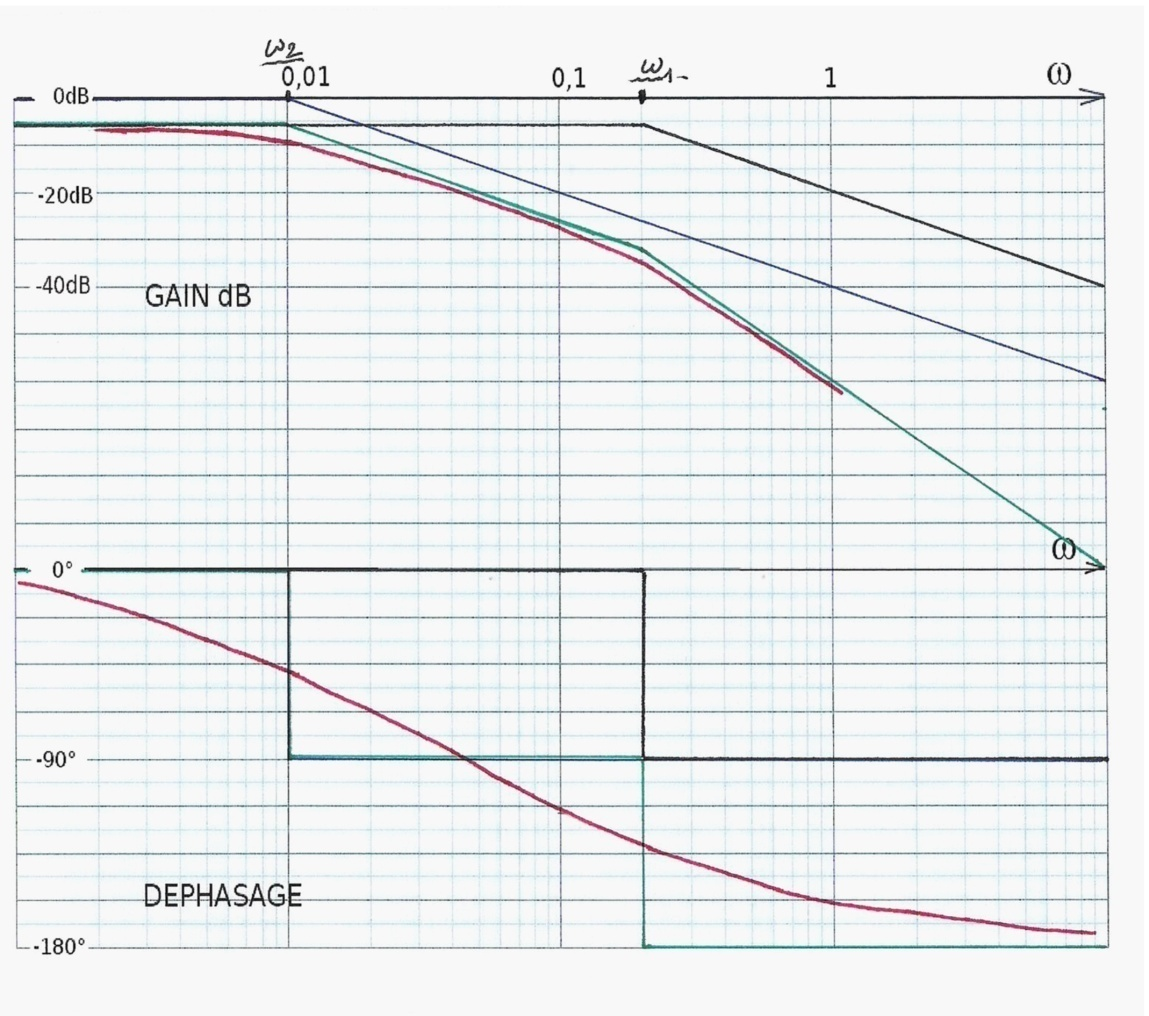
\includegraphics[width=6.00972in,height=5.31181in]{pandoc/images/image15.jpeg}

\textbf{En considérant uniquement le terme proportionnel du correcteur, déterminer, en le justifiant, la valeur de K permettant d'obtenir une marge de phase de 70°.}

\textbf{Déterminer la valeur de T\textsubscript{i} pour que la marge de phase obtenue précédemment ne soit pas dégradée de plus de 5°.}
\end{minipage} \\
\midrule\noalign{}
\endhead
\bottomrule\noalign{}
\endlastfoot
\end{longtable}

\hypertarget{retard-de-phase-ou-correcteur-pi-ruxe9el}{%
\section{\texorpdfstring{ retard de phase (ou correcteur PI réel)}{ retard de phase (ou correcteur PI réel)}}\label{retard-de-phase-ou-correcteur-pi-ruxe9el}}

\TLBodeRetardPhase[1][10][1]


Le correcteur PI est censé avoir un gain infini aux basses fréquences. Si les puissances en jeu sont trop importantes, il est impossible de réaliser concrètement ce comportement théorique. Le correcteur à retard de phase exerce une action intégrale limitée à une plage de fréquence. Ce correcteur augmente le gain de la FTBO aux basses fréquences et modifie la précision du système. Le correcteur à retard de phase enlève de la phase.

Le correcteur \textbf{à retard de phase} \(C(p) = K\frac{1 + \tau_{i}p}{1 + a\tau_{i}p}\)~, avec \(a > 1\) :

\begin{itemize}
\item
  \textbf{améliore la précision mais dégrade la stabilité~;}
\item
  \textbf{augmente le gain aux basses fréquences.}
\end{itemize}

Diagramme de Bode du correcteur à retard de phase~:

La phase est minimale pour \(\omega_{\min} = \frac{1}{\sqrt{a}\tau_{i}}\) et vaut \(\sin\varphi_{\min} = \frac{1 - a}{1 + a}\) .

Calcul de la moyenne logarithmique entre \(\frac{1}{\tau_{i}}\) et \(\frac{1}{a\tau_{i}}\)

\[\log\omega_{\min} = \frac{1}{2}\left( \log\frac{1}{\tau_{i}} + \log\frac{1}{a\tau_{i}} \right) = \log\left( \sqrt{\frac{1}{\tau_{i}}.\frac{1}{a\tau_{i}}} \right) = \log\left( \frac{1}{\sqrt{a}\tau_{i}} \right)\  \Rightarrow \omega_{\min} = \frac{1}{\sqrt{a}\tau_{i}}\]

\hypertarget{stabilituxe9-3}{%
\subsubsection*{Stabilité}\label{stabilituxe9-3}}
\addcontentsline{toc}{subsubsection}{Stabilité}

La stabilité est plutôt diminué vu que l'on enlève de la phase. Cependant, en choisissant bien K, on peut la préserver. Parfois même, on peut augmenter les marges en diminuant \(\omega_{0dB}\).

\hypertarget{rapidituxe9-3}{%
\subsubsection*{Rapidité}\label{rapidituxe9-3}}
\addcontentsline{toc}{subsubsection}{Rapidité}

A l'inverse, la rapidité diminue.

\hypertarget{pruxe9cision-3}{%
\subsubsection*{Précision}\label{pruxe9cision-3}}
\addcontentsline{toc}{subsubsection}{Précision}

La précision est améliorée sans changer la classe. Donc les écarts statiques sont réduits mais ne sont pas annulés.

\hypertarget{ruxe9glage-du-correcteur-1}{%
\subsubsection*{Réglage du correcteur}\label{ruxe9glage-du-correcteur-1}}
\addcontentsline{toc}{subsubsection}{Réglage du correcteur}

Si on choisit \(K = a\) le gain est nul pour les hautes fréquences.

On règle ce correcteur pour augmenter le gain aux basses fréquences sans diminuer la phase au voisinage du point critique.

\hypertarget{correcteur-duxe9rivuxe9-d-et-proportionnel-duxe9rivuxe9-pd}{%
\section{Correcteur dérivé D et proportionnel dérivé PD}\label{correcteur-duxe9rivuxe9-d-et-proportionnel-duxe9rivuxe9-pd}}

Le correcteur \textbf{dérivé} \(C(p) = K_{d}p\) et le correcteur \textbf{proportionnel dérivé} \(C(p) = K_{p} + K_{d}p\) ne sont pas réalisables technologiquement. Ils ont un degré du numérateur supérieur à celui du dénominateur. Ils ajoutent un zéro à la FTBO sans changer la classe. Pour réaliser ces correcteurs, il faut avoir une amplification très importante pour les très hautes fréquences, ce qu'aucun système physique ne permet. Les réalisations essayant d'approcher ces modèles théoriques amplifient tous les bruits et leurs grandeurs de sortie sont inexploitables.

Correcteur PD théorique

\hypertarget{correcteur-uxe0-avance-de-phase-ou-correcteur-pd-ruxe9el}{%
\subsection{Correcteur à avance de phase (ou correcteur PD réel)}\label{correcteur-uxe0-avance-de-phase-ou-correcteur-pd-ruxe9el}}

\TLBodeAvancePhase[1][0.1][1]


Le correcteur à avance de phase fait exactement l'inverse du correcteur à retard de phase. C'est la seule utilisation pratique de l'action dérivée.

Il fait une action dérivée sur une plage de fréquence.

Le correcteur à avance de phase ajoute de la phase.

Le correcteur \textbf{à avance de phase} \(C(p) = K\frac{1 + T_{d}p}{1 + aT_{d}p}\)~, avec \(a < 1\) :

\begin{itemize}
\item
  \textbf{augmente la stabilité mais introduit des vibrations et du bruit~;}
\item
  \textbf{améliore la rapidité}.
\end{itemize}

Diagramme de Bode du correcteur à avance de phase~:

La phase est maximale pour \(\omega_{\max} = \frac{1}{\sqrt{a}T_{d}}\ \ \) et vaut \(\sin\varphi_{\max} = \frac{1 - a}{1 + a}\) .

\hypertarget{stabilituxe9-4}{%
\subsubsection*{Stabilité}\label{stabilituxe9-4}}
\addcontentsline{toc}{subsubsection}{Stabilité}

Ce correcteur augmente la marge de phase autour du point critique et peut stabiliser un système instable ou augmenter les marges.

\hypertarget{rapidituxe9-4}{%
\subsubsection*{Rapidité}\label{rapidituxe9-4}}
\addcontentsline{toc}{subsubsection}{Rapidité}

Le gain des hautes fréquences est augmenté, donc la bande passante est plus large et la rapidité est amélioré.

\hypertarget{pruxe9cision-4}{%
\subsubsection*{Précision}\label{pruxe9cision-4}}
\addcontentsline{toc}{subsubsection}{Précision}

La précision diminue en fonction des valeurs choisies.

\hypertarget{ruxe9glage-du-correcteur-2}{%
\subsubsection*{Réglage du correcteur}\label{ruxe9glage-du-correcteur-2}}
\addcontentsline{toc}{subsubsection}{Réglage du correcteur}

\begin{itemize}
\item
  On cherche la valeur a qui permet d'obtenir \(M_{\varphi}\) demandée avec \(\sin\varphi_{\max} = \frac{1 - a}{1 + a}\).
\item
  On cherche \(\tau_{d}\) avec \(\omega_{\max} = \omega_{0db}\) soit \(\tau_{d} = \frac{1}{\sqrt{a}\omega_{0dB}}\).
\item
  On ajuste K pour que le gain du système corrigé soit bien de 0dB pour \(\omega_{\max}\).
\end{itemize}

\hypertarget{correcteur-proportionnel-intuxe9gral-duxe9rivuxe9-pid}{%
\section{Correcteur proportionnel intégral dérivé PID}\label{correcteur-proportionnel-intuxe9gral-duxe9rivuxe9-pid}}

\TLBodeCorrecteurPID[1][10][1][0.1]


Il se comporte comme un correcteur intégral pour les basses fréquences et comme un correcteur proportionnel pour les fréquences intermédiaires et comme un correcteur dérivé pour les hautes fréquences. Bien réglé, il présente les avantages 3 correcteurs sans leurs inconvénients. Mais il est difficile à régler.

Le correcteur \textbf{proportionnel intégral dérivé} \(C(p) = K_{p} + \frac{K_{i}}{p} + K_{d}p\)~:

\begin{itemize}
\item
  Comme le correcteur PI, il améliore la précision~;
\item
  Comme le correcteur PD, il améliore la rapidité.
\end{itemize}

Correcteur PID théorique

Ce correcteur ne correspond à aucun système physique car le degré du numérateur est supérieur à celui du dénominateur.

Les correcteurs réels que l'on utilise sont de la forme~:

\(C(p) = K\frac{1 + \tau_{i}p}{\tau_{i}p}\frac{1 + \tau_{d}p}{1 + b\tau_{d}p}\) ou \(C(p) = K\frac{1 + \tau_{i}p}{1 + a\tau_{i}p}\frac{1 + \tau_{d}p}{1 + b\tau_{d}p}\) avec \(a > 1\) et \(b < 1\)

Diagramme de Bode du correcteur PID~:

\hypertarget{ruxe9glage-du-correcteur-3}{%
\subsubsection*{Réglage du correcteur}\label{ruxe9glage-du-correcteur-3}}
\addcontentsline{toc}{subsubsection}{Réglage du correcteur}

\begin{itemize}
\item
  On commence par la rapidité et de précision avec le correcteur PI.
\item
  Puis la stabilité avec l'avance de phase.
\end{itemize}

Ziegler et Nichols ont proposé deux approches heuristiques basées sur leur expérience et quelques simulations pour ajuster rapidement les paramètres des régulateurs P, PI et PID.

La première méthode nécessite l\textquotesingle enregistrement de la réponse indicielle en boucle ouverte, alors que la deuxième demande d\textquotesingle amener le système bouclé à sa limite de stabilité.

Il existe bien d'autres méthodes, mais qui ne sont pas détaillées ici car hors programme.

\hypertarget{bilan-des-performances-des-correcteurs}{%
\section{Bilan des performances des correcteurs}\label{bilan-des-performances-des-correcteurs}}

La problématique des asservissements est de trouver le meilleur \textbf{compromis} entre les différentes performances.

\begin{longtable}[]{@{}
  >{\raggedright\arraybackslash}p{(\columnwidth - 6\tabcolsep) * \real{0.4671}}
  >{\raggedright\arraybackslash}p{(\columnwidth - 6\tabcolsep) * \real{0.1775}}
  >{\raggedright\arraybackslash}p{(\columnwidth - 6\tabcolsep) * \real{0.1779}}
  >{\raggedright\arraybackslash}p{(\columnwidth - 6\tabcolsep) * \real{0.1775}}@{}}
\toprule\noalign{}
\begin{minipage}[b]{\linewidth}\raggedright
\textbf{Performances}
\end{minipage} & \begin{minipage}[b]{\linewidth}\raggedright
\textbf{Stabilité}
\end{minipage} & \begin{minipage}[b]{\linewidth}\raggedright
\textbf{Rapidité}
\end{minipage} & \begin{minipage}[b]{\linewidth}\raggedright
\textbf{Précision}
\end{minipage} \\
\midrule\noalign{}
\endhead
\bottomrule\noalign{}
\endlastfoot
Correcteur P & \(\searrow\) & \(\nearrow \nearrow\) & \(\nearrow\) \\
Correcteur I & \(\searrow \searrow\) & \(\searrow\) & \(\nearrow \nearrow\) \\
Correcteur PI & \(\searrow\) & \(\searrow\) & \(\nearrow \nearrow\) \\
Correcteur à retard de phase & \(\searrow\) & \(\searrow\) & \(\nearrow\) \\
Correcteur à avance de phase & \(\nearrow\) & \(\nearrow\) & \(\searrow\) \\
Correcteur PID & \(\nearrow\) & \(\nearrow\) & \(\nearrow \nearrow\) \\
\end{longtable}

\hypertarget{ruxe9gulation-cascade-ou-boucles-imbriquuxe9es}{%
\section{Régulation cascade ou boucles imbriquées}\label{ruxe9gulation-cascade-ou-boucles-imbriquuxe9es}}

\TLBouclesImbriquees


Afin d'améliorer la robustesse de notre système, des boucles imbriquées ou régulation cascade sont souvent utilisées. Le principe est d'asservir une grandeur et sa dérivée comme par exemple la position et la vitesse. Pour cela il faut que le temps de réponse de la boucle interne soit négligeable devant la boucle externe.

\textbf{Exemple de boucle de vitesse et de position}


\includegraphics[width=2.52778in,height=1.81528in]{pandoc/images/image16.jpeg}Pour minimiser l\textquotesingle effet des non-linéarités du moteur et lutter plus efficacement contre les perturbations qui affectent l\textquotesingle ensemble du processus, le moteur va être asservi en vitesse puis en position à l\textquotesingle aide d\textquotesingle un capteur placé sur son arbre de sortie.

Le moteur étant asservi en courant, on réalise les deux boucles imbriquées suivantes :


\includegraphics[width=5.91667in,height=2.39583in]{pandoc/images/image9.png}

Cela a plusieurs avantages~:

\begin{itemize}
\item
  La boucle interne (ici de vitesse) permet de minimiser les non linéarités (comme tout système bouclé).
\item
  La régulation cascade rend le système plus rapide car le bouclage interne permet «~d'anticiper~» les fluctuations que ce soit au niveau de la consigne ou des perturbations
\item
  La robustesse est bien meilleure car les deux asservissements permettent de corriger les perturbations et incertitudes sur les modèles.
\end{itemize}

Pour régler cet asservissement, on commence par régler la boucle interne de manière à ce qu'elle soit la plus rapide possible. Ensuite, on s'occupe de la boucle externe.

\hypertarget{sources}{%
\section{Sources}\label{sources}}

Ce cours a été élaboré à l'aide de nombreuses ressources~provenant de différents collègues~de l'UPSTI.\\


\clearpage
\section{Exercices du chapitre}\label{exercices-correction-sa}
% Exercices issus de 10-CorrectionSA2022.docx.

\includegraphics[width=5.46667in,height=8.37353in]{pandoc/images/image17.png}

\hypertarget{ruxe9gler-un-correcteur-proportionnel}{%
\subsection{Régler un correcteur proportionnel}\label{ruxe9gler-un-correcteur-proportionnel}}


\includegraphics[width=1.35556in,height=0.38889in]{pandoc/images/image18.png}\textbf{~}\protect\hypertarget{_Toc120222132}{}{}\textbf{Marges de stabilité et correcteur P}

Soit \(F(p)\) la FTBO d'un système bouclé à retour unitaire d'entrée \(x(t)\) et de sortie \(y(t)\). Les diagrammes de BODE de \(F(p)\) sont représentés ci-dessous.


\includegraphics[width=4.6875in,height=2.8125in]{pandoc/images/image19.png}


\includegraphics[width=4.75in,height=2.33333in]{pandoc/images/image20.png}

Diagrammes de BODE de la FTBO

Tracer le schéma-bloc du système asservi.

Déterminer les marges de phase et de gain du système, puis conclure quant à sa stabilité.

On décide d'ajouter au système un correcteur série de type proportionnel. On note K le gain de ce correcteur.

Déterminer la valeur de K permettant d'obtenir une marge de gain \(M_{G} = 12\ dB\).

Déterminer la nouvelle marge de phase du système et conclure quant à sa stabilité.

En précisant la méthode permettant de le calculer, déterminer l'écart statique \(\varepsilon_{s}\) du système corrigé pour une entrée indicielle.

\textbf{~}\protect\hypertarget{_Toc120222133}{}{}\textbf{Axe de robot}

La commande d'axe d'un robot est décrite par le schéma-bloc ci-dessous.


\includegraphics[width=7.22917in,height=1.85417in]{pandoc/images/image21.png}

Schéma bloc de la commande d'un axe de robot

avec :

• \(C(p)\) : fonction de transfert du correcteur

• \(M(p) = \frac{k}{RJp + k^{2}}\) : modélisation du moteur à courant continu

--- \(R\) : résistance totale \(\lbrack\Omega\rbrack\)

--- \(J\) : moment d'inertie équivalent ramené sur l'axe de rotation \(\lbrack kg.m^{2}\rbrack\)

--- \(k\) : constante de couple {[}N.m/A{]} et constante de vitesse \(\lbrack V/(rad/s)\rbrack\)

• \(\lambda\) : rapport de réduction

• \(G_{T}\) : gain de la génératrice tachymétrique \(\lbrack V/(rad/s)\rbrack\)

• \(K_{C}\) : gain de l'amplificateur de puissance

• \(K_{\alpha}\) : gain du capteur de position \(\lbrack V/rad\rbrack\)

Afin d'assurer une mise en position correcte, on ne veut aucun écart de position. Quant à l'écart de traînage il est limité à 1\%.

Déterminer la fonction de transfert en boucle ouverte, notée \(B(p)\), de cette commande d'axe.

Conclure sur la possibilité de pouvoir respecter les critères imposés par le cahier des charges en termes de précision avec un correcteur proportionnel.

\textbf{~}\protect\hypertarget{_Toc120222134}{}{}\textbf{Asservissement de vitesse}

On propose le schéma-bloc d'un asservissement d'un dispositif régulant la vitesse \(\omega\) d'un moteur perturbé par un couple résistant \(c_{r}(t)\).


\includegraphics[width=7.22917in,height=1.64583in]{pandoc/images/image22.png}


\includegraphics[width=3.67361in,height=2.46181in]{pandoc/images/image23.png}Schéma bloc de l'asservissement de vitesse

Où~:

\begin{itemize}
\item
  \(G_{T}\) : gain de la génératrice tachymétrique et du transducteur de consigne, avec \(G_{T} = 0,08\ V\text{/}\left( rad\text{/}s \right)\)
\item
  \(C(p)\) : fonction de transfert du correcteur
\item
  \(A\) : gain de l'amplificateur avec A = 30
\item
  \(K_{T}\) : constante de couple du moteur
\item
  \(K_{E}\) : constante de force contre électromotrice du moteur
\item
  \(R\) : résistance de l'induit
\item
  \(L\) : inductance de l'induit
\item
  \(J\) : moment d'inertie du rotor par rapport à son axe de rotation
\item
  \(f\) : paramètre de frottement visqueux
\end{itemize}

FIGURE 4 -- Réponse à un échelon de consigne : 10 rad/s

La figure 4 fournit la réponse indicielle du dispositif non perturbé avec un correcteur proportionnel de gain \(K = 1\).

Déterminer l'erreur statique et l'erreur statique relative en régime permanent.

A partir de la réponse, déterminer le gain de la FTBO.

On souhaite une erreur statique relative inférieure à 1 \% ; quelle valeur doit-on donner au gain du correcteur ? Quel problème peut poser la valeur du gain ainsi déterminée ?

On considère à présent une perturbation en échelon d'amplitude \(C_{R0} = 100\ Nm\).

La perturbation provoque-t-elle une erreur supplémentaire en régime permanent ? donner sa valeur.

Quelle proposition peut-on faire pour améliorer la précision de cet asservissement de vitesse ?

\protect\hypertarget{_Toc120222135}{}{}\textbf{Commande de gouverne}

Le dispositif étudié régule la position angulaire d'une gouverne de profondeur d'avion. Il est schématisé sur la figure 1 ci-dessous~:


\includegraphics[width=2.08333in,height=1.38472in]{pandoc/images/image24.png}
\includegraphics[width=4.525in,height=1.96994in]{pandoc/images/image25.png}

FIGURE 1 -- Gouverne en position horizontale

La rotation de cette gouverne est assurée par le déplacement \(x\) de la tige d'un vérin hydraulique actif provoqué par un débit \(q\). Un vérin passif est chargé de l'amortissement du mouvement.

Cette mise en position est perturbée par des effets aérodynamiques, modélisés par la force \(F_{A}\).

Pour être dans le cadre des systèmes linéaires, on se place autour d'un point de fonctionnement, celui de la figure proposée.

À partir de l'équation de débit du vérin actif et de l'équation obtenue par le théorème de l'énergie cinétique appliqué à l'ensemble \(\{ gouverne,\ vérins\}\), on peut tracer le schéma-bloc de la figure 2.


\includegraphics[width=5.1875in,height=2.08333in]{pandoc/images/image26.png}

FIGURE 2 -- Schéma-bloc de la commande non asservie de la position de la tige du vérin

Sur ce schéma-bloc sont notés :

• \(B\) : module de compressibilité du fluide

• \(V_{0}\) : volume de la chambre du vérin


\includegraphics[width=2.60833in,height=1.65903in]{pandoc/images/image27.png}• \(S\) : section utile du vérin

• \(m\) : masse de la tige du vérin

• \(\mu\) : paramètre d'amortissement visqueux

• \(h = \overrightarrow{BC}.\overrightarrow{y}\)

• \(H = \overrightarrow{BM}.\overrightarrow{x}\)

Déterminer les fonctions de transfert \(G(p)\) et \(W(p)\) telles que le schéma proposé puisse se mettre sous la forme de la figure 3.

\begin{quote}
FIGURE 3 -- Schéma-bloc équivalent
\end{quote}

On réalise un asservissement de la position \(x\) de la tige tel que décrit sur la figure 4. Le débit est délivré par une servovalve commandée en courant. À partir de l'écart, un amplificateur proportionnel de gain \(C\) fournit le courant \(i\) d'alimentation de la bobine de la servovalve. La mesure de la position de la tige du vérin actif est réalisée par un capteur de gain \(K_{M}\).


\includegraphics[width=5.875in,height=2.0625in]{pandoc/images/image28.png}

FIGURE 4 -- Schéma-bloc de la commande asservie

Le cahier des charges impose en régime permanent :

• une erreur nulle pour une entrée de consigne en échelon ;

• un écart inférieur ou égal à \(2mm\) si \(x_{c}(t)\  = \ 0,1\ t\).

Quel nom donner au bloc contenant \(A(p)\) et quelle fonction de transfert faut-il y poser ? Justifier la réponse.

Montrer qu'en régime permanent, le signal de sortie n'est pas affecté par une perturbation en échelon de force d'amplitude \(F_{0}\).

En absence de perturbation, on peut modéliser l'asservissement de position par le schéma-bloc de la figure 5 ci-dessous.


\includegraphics[width=5.45833in,height=0.875in]{pandoc/images/image29.png}

FIGURE 5 -- Schéma-bloc sans perturbation

Quelle expression doit prendre le gain de boucle afin de satisfaire aux exigences du cahier des charges concernant la précision ?

\hypertarget{ruxe9gler-un-correcteur-intuxe9gral}{%
\subsection{Régler un correcteur intégral}\label{ruxe9gler-un-correcteur-intuxe9gral}}

\protect\hypertarget{_Toc120222136}{}{}\textbf{Asservissement en vitesse angulaire d'un moteur électrique}

L'asservissement de vitesse d'un moteur électrique est représenté par le schéma fonctionnel ci-dessous :


\includegraphics[width=4.58333in,height=0.875in]{pandoc/images/image30.png}

Le gain \(A\ \)du hacheur est de \(A = 1\ V/(rad/s)\)

La fonction de transfert du moteur est \(H(p) = \frac{1}{(1 + 0,08p)(1 + 0,002p)}\)

Le cahier des charges impose :

\begin{itemize}
\item
  une marge de phase de 45° ;
\item
  une erreur en régime permanent nulle, vis-à-vis d'une consigne en échelon.
\end{itemize}

Objectif :

− évaluer les performances de cet asservissement ;

− régler les paramètres d'un correcteur permettant le respect des critères du cahier des charges.

Déterminer les marges du système non corrigé.

Déterminer l'erreur en régime permanent du système non corrigé pour une consigne en échelon d'amplitude \(\omega_{c0}.\)

Conclure.

On utilise maintenant un correcteur \(C(p) = K_{p} + \frac{K_{i}}{p} = K_{p}\frac{1 + T_{i}p}{T_{i}p}\) avec \(T_{i} = \frac{K_{p}}{K_{i}}\).

Quelle est la nature de ce correcteur ? Que peut-on attendre comme amélioration sur le système ?

Tracer le diagramme de Bode asymptotique de ce correcteur pour \(K_{p} > 1\). Indiquer les caractéristiques~:

\begin{itemize}
\item
  pentes des asymptotes ;
\item
  expressions de la pulsation, du gain en dB et de la phase au point de cassure.
\end{itemize}

\emph{Compléter avec l'allure des courbes réelles.}

Le lieu de Bode de la fonction de transfert en boucle ouverte non corrigée est donné ci-après.

Déterminer graphiquement puis analytiquement les paramètres \(K_{p} > 1\) et \(K_{i} > 1\) du correcteur par la méthode du placement fréquentiel.

Déterminer les paramètres \(K_{p} > 1\) et \(K_{i} > 1\) du correcteur par la méthode de la compensation du pôle dominant.


\includegraphics[width=4.14583in,height=2.8125in]{pandoc/images/image31.png}


\includegraphics[width=4.20833in,height=2.33333in]{pandoc/images/image32.png}

On construit le modèle causal du servomoteur~:


\includegraphics[width=5.45833in,height=1.29167in]{pandoc/images/image33.png}

On donne la réponse temporelle du système non corrigé et des réglages précédant~:


\includegraphics[width=5.375in,height=3.25in]{pandoc/images/image34.png}

Quel est le meilleur réglage.

\hypertarget{reglage-dun-correcteur-pi}{%
\subsection{~REGLAGE D'un correcteur pi}\label{reglage-dun-correcteur-pi}}

Un système est corrigé par un correcteur de type P.I.


\includegraphics[width=4.41181in,height=0.86806in]{pandoc/images/image35.jpeg}

On suppose \(K_{p} > 0.\)

Pour le réglage du correcteur, on hésite entre \(T_{i} = 0,5s\) et \(T_{i} = 5s\).

Déterminer la FTBF dans les deux cas, mettre sous forme canonique puis exprimer les paramètres caractéristiques des fonctions de transfert.

\textbf{Réglage en commençant par la stabilité}

On souhaite un coefficient d'amortissement \(z = 0,5\).

Déterminer \(K_{p}\) pour chacun des cas.

Déterminer alors la largeur de la bande passante à -3dB pour chacun des cas.


\includegraphics[width=3.45347in,height=2.59375in]{pandoc/images/image36.png}On donne la réponse temporelle pour un échelon d'amplitude 10 de ces 2 correcteurs ci-dessous~:


\includegraphics[width=3.53333in,height=1.28194in]{pandoc/images/image37.png}

Conclure.

\textbf{Réglage en commençant par la rapidité}

On souhaite une pulsation de coupure \(\omega_{- 3dB} = 1\ rad/s\).

Déterminer \(K_{p}\) pour chacun des cas.

Déterminer alors le coefficient d'amortissement pour chacun des cas.

Conclure.

\textbf{Comparaison}

Conclure sur le réglage du correcteur PI.

\hypertarget{ruxe9gler-un-correcteur-uxe0-avance-de-phase}{%
\subsection{Régler un correcteur à avance de phase}\label{ruxe9gler-un-correcteur-uxe0-avance-de-phase}}

\protect\hypertarget{_Toc120222138}{}{}\textbf{Correcteur a avance de phase du robovolc}

(D'après E3A PSI 2017)


\includegraphics[width=2.06319in,height=1.55139in]{pandoc/images/image38.png}On s'intéresse au véhicule Robovolc, un robot qui explore le flanc des volcans. Ce robot est capable de :

\begin{itemize}
\item
  s\textquotesingle approcher d\textquotesingle un cratère actif ;
\item
  collecter des échantillons rocheux issus de rejets éruptifs ;
\item
  collecter des échantillons gazeux ;
\item
  collecter d\textquotesingle autres données physiques et chimiques.
\end{itemize}

~Tracer le diagramme de Bode asymptotique de la fonction \(H(p) = \frac{\delta\tau_{B}p + 1}{\tau_{B}p + 1}\) avec \(\delta > 1\)

~Quel est l'intérêt de ce correcteur à avance de phase~?

~En utilisant une moyenne logarithmique entre \(\frac{1}{\delta\tau_{B}}\) et \(\frac{1}{\tau_{B}}\) montrer que la valeur maximale de la phase à lieu pour \(\omega_{maxi} = \frac{1}{\sqrt{\delta}.\tau_{B}}\)

Déterminer \(\delta\) tel que \(\varphi\left( \omega_{maxi} \right) = 45{^\circ}\)

On étudie l'asservissement d'une MSAP, on donne la fonction suivante~:

\[{FTBO}_{corr\Omega}(p) = K_{pi}\ \frac{\delta\ \tau_{B}\ p + 1}{\delta.\tau_{B}\ p}\frac{B}{p(1 + \tau_{B}p)}\]

Avec \(\delta = 5,83\), \(B = 45\ (rad/s)^{2}/A\), \(\tau_{B} = 33,87\ ms\)

Déterminer \(K_{pi}\) tel que \(G_{dB}\left( \omega_{maxi} \right) = 0dB\). Quel est l'intérêt~?


\includegraphics[width=0.92361in,height=0.63819in]{pandoc/images/image39.jpeg}

\textbf{Autour de la bande passante}

\emph{(\ul{Source :} Marc Dérumaux)}

On considère la FTBO dont le diagramme de Bode est tracé ci-dessous, à gauche pour une large gamme de fréquence et à droite pour une gamme de fréquence plus étroite :


\includegraphics[width=4.24306in,height=3.1875in]{pandoc/images/image40.emf}
\includegraphics[width=3.88889in,height=2.75694in]{pandoc/images/image41.emf}

\begin{enumerate}
\def\labelenumi{\arabic{enumi}.}
\item
  Quelle sont les valeurs des marges de gain et de phase ?
\item
  Quelle est la bande passante à 0dB ?
\item
  Quelle correction proportionnelle Kp1 faut-il choisir pour assurer une bande passante de 0.6 rad/s ?
\item
  Quelle correction proportionnelle Kp2 faut-il choisir pour assurer une marge de gain de 6dB ?
\item
  Quelle correction proportionnelle Kp3 faut-il choisir pour assurer une marge de phase de 60° ?
\item
  Si le cahier des charges impose une bande passante d\textquotesingle au moins 0.6 rad/s, une marge de gain d\textquotesingle au moins 12 dB et une marge de phase d\textquotesingle au moins 60°, quelle correction proportionnelle Kp faut-il choisir ?
\end{enumerate}

